% Slide 28: Non-linear Problems
\begin{frame}{مسائل غیرخطی در رگرسیون}{\lr{Non-linear Problems}}
  \begin{columns}[T]
    \begin{column}{0.54\textwidth}
      \begin{itemize}
        \setlength{\itemsep}{6pt}
        \item بسیاری از فرآیندهای واقعی از برازش خط مستقیم پیروی نمی‌کنند.
        \item \textbf{راهکارهای اساسی مدل‌سازی غیرخطی:}
        \begin{itemize}
          \setlength{\itemsep}{4pt}
          \item \textbf{رگرسیون هم‌نوا یا ایزوتونیک} (\lr{Isotonic})؛ برای توابع غیرخطی اما یکنواخت (صعودی یا نزولی).
          \item \textbf{رگرسیون چندجمله‌ای} (\lr{Polynomial})؛ برای برازش منحنی‌های پیچیده و غیریکنواخت.
        \end{itemize}
      \end{itemize}
    \end{column}
    \begin{column}{0.44\textwidth}
      \begin{center}
        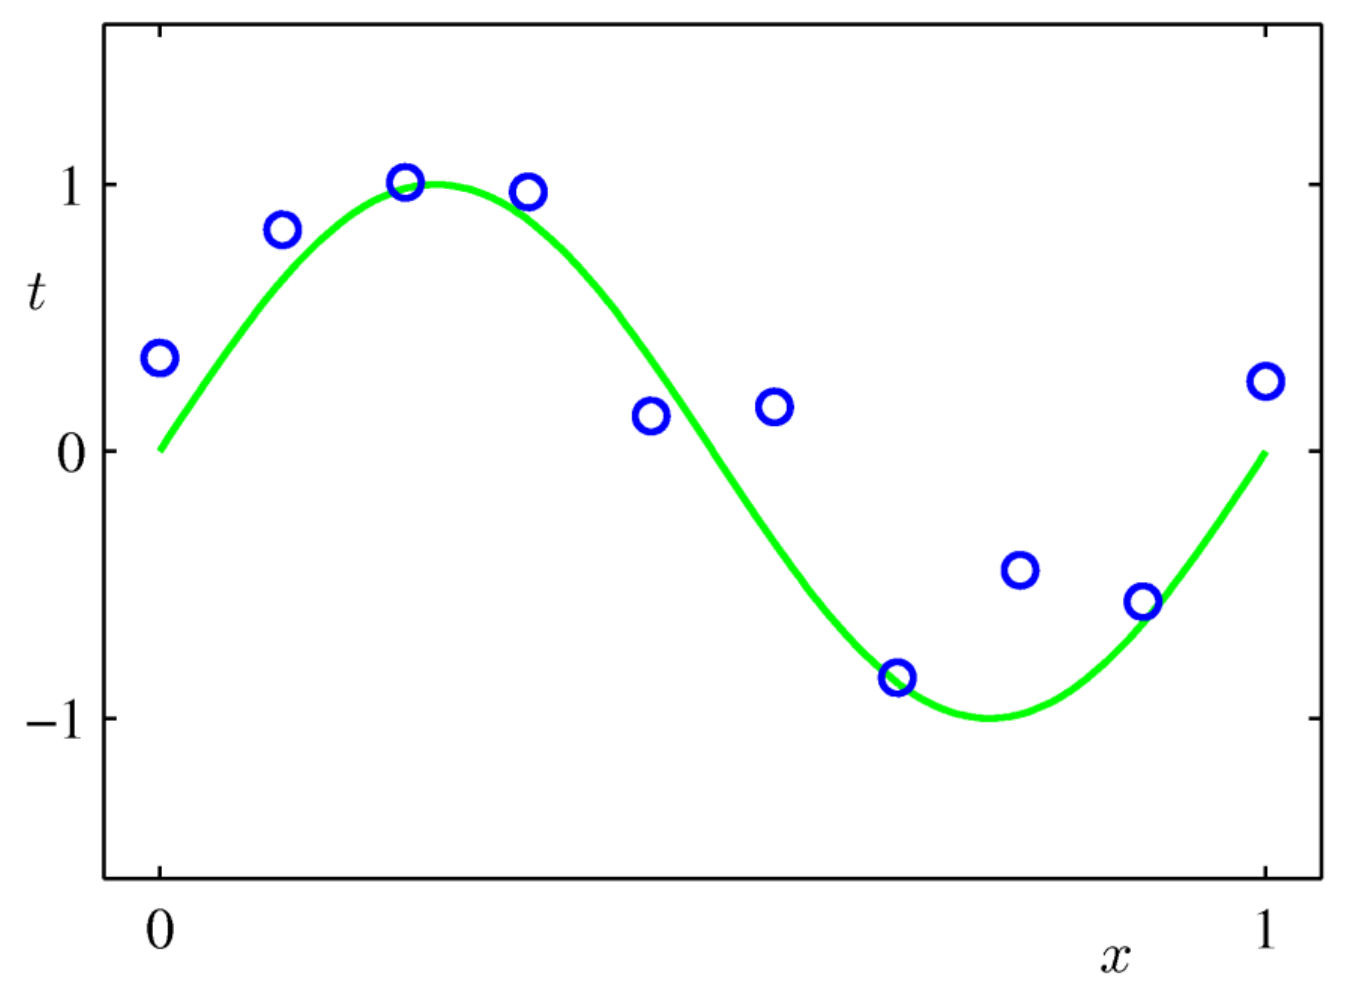
\includegraphics[width=\textwidth,height=4.0cm,keepaspectratio]{images/slide28_nonlinear_curve.png}
      \end{center}
    \end{column}
  \end{columns}
\end{frame}

% Slide 29: Isotonic Regression
\begin{frame}{رگرسیون هم‌نوا (ایزوتونیک)}{\lr{Isotonic Regression}}
  \begin{itemize}
    \setlength{\itemsep}{6pt}
    \item \textbf{حالت خاص:} تابع هدف \textbf{یکنواخت یا هم‌نوا (\lr{Monotonous})} است.
    \item اگر $x_1 \le x_2$ باشد، آنگاه رابطه $f(x_1) \le f(x_2)$ ارضا می‌شود:
    \[
      x_1 \le x_2 \implies f(x_1) \le f(x_2)
    \]
    \item برای این دسته از مسائل، الگوریتم‌های بهینه‌سازی بسیار سریعی توسعه یافته است.
    \item \textbf{ساده‌ترین و پرکاربردترین روش:}
    \textbf{الگوریتم تجمیع متجاوزان مجاور (\lr{Pool Adjacent Violators Algorithm - PAVA})}.
  \end{itemize}
\end{frame}

% Slide 30: PAVA Step 1
\begin{frame}{\rl{الگوریتم تجمیع متجاوزان مجاور: گام ۱}}{\lr{Pool Adjacent Violators: Step 1}}
  \begin{itemize}
    \setlength{\itemsep}{2pt}
    \item شناسایی متجاوزان مجاور (\lr{Adjacent Violators})؛ نقاطی که در آن‌ها $f(x_i) > f(x_{i+1})$.
    \item جایگزینی با مقادیر $f'(x_i) = f'(x_{i+1})$ به گونه‌ای که مجموع مربعات خطا کمینه شود.
    \item تجمیع نقاط (اصطلاحاً \lr{Pool})، به طوری که از این پس به عنوان یک نقطه واحد در نظر گرفته می‌شوند.
    \item تکرار تا زمانی که هیچ متجاوز مجاوری باقی نماند.
  \end{itemize}
  \vspace{-0.1cm}
  \begin{center}
    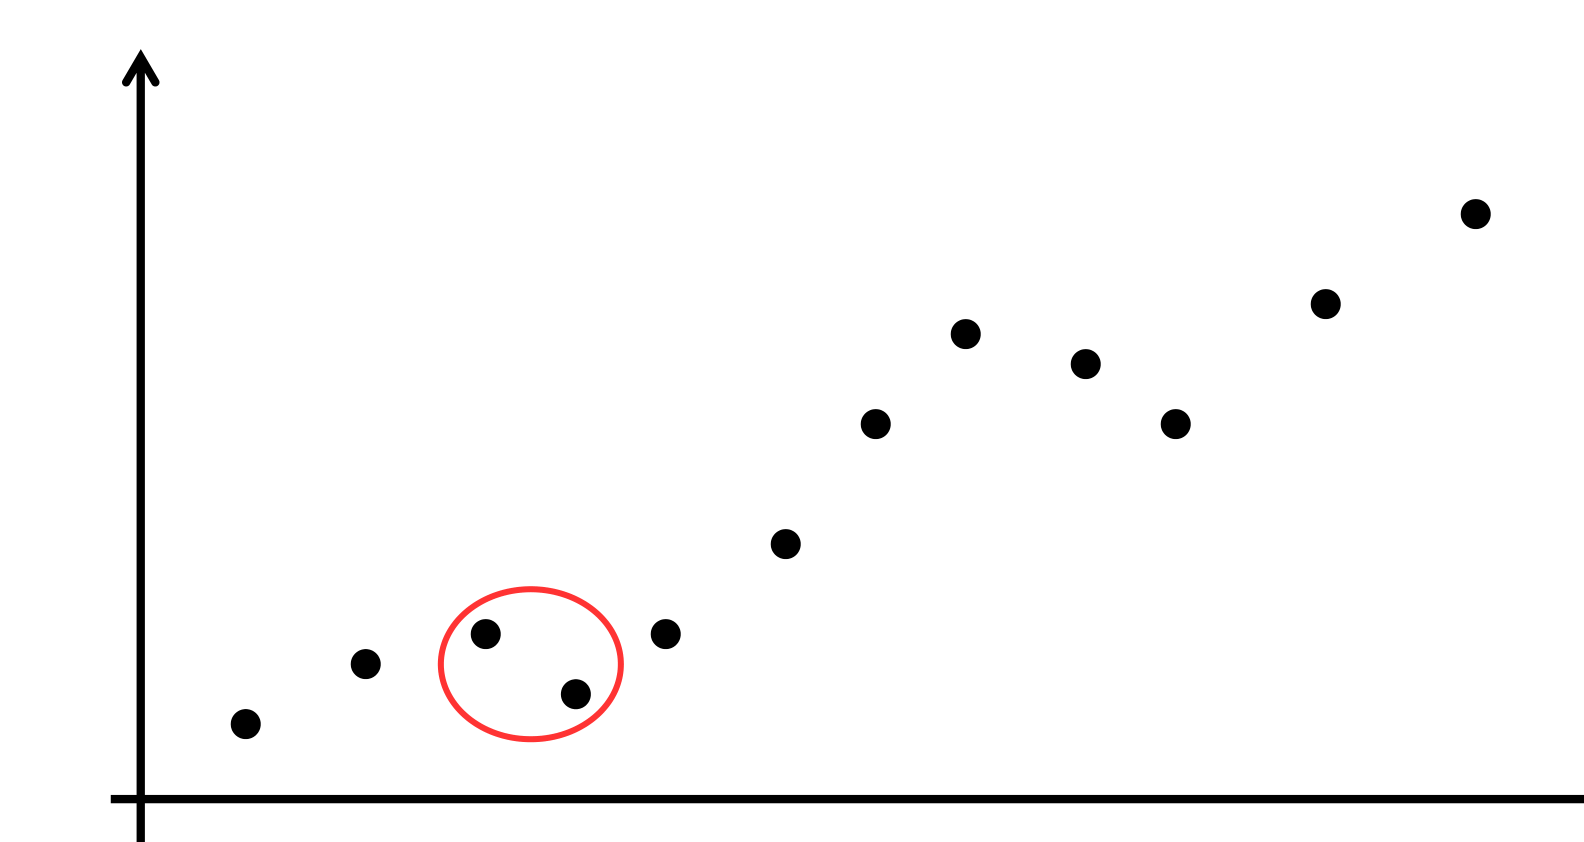
\includegraphics[height=3.0cm,keepaspectratio]{images/slide30_isotonic_step1.png}
  \end{center}
\end{frame}

% Slide 31: PAVA Step 2
\begin{frame}{\rl{الگوریتم تجمیع متجاوزان مجاور: گام ۲}}{\lr{Pool Adjacent Violators: Step 2}}
  \begin{itemize}
    \setlength{\itemsep}{3pt}
    \item ادغام نقاط مرحله قبل و یافتن جفت متجاوز مجاور بعدی.
    \item محاسبه میانگین جدید جهت حفظ بهینگی مجموع مربعات خطا.
  \end{itemize}
  \begin{center}
    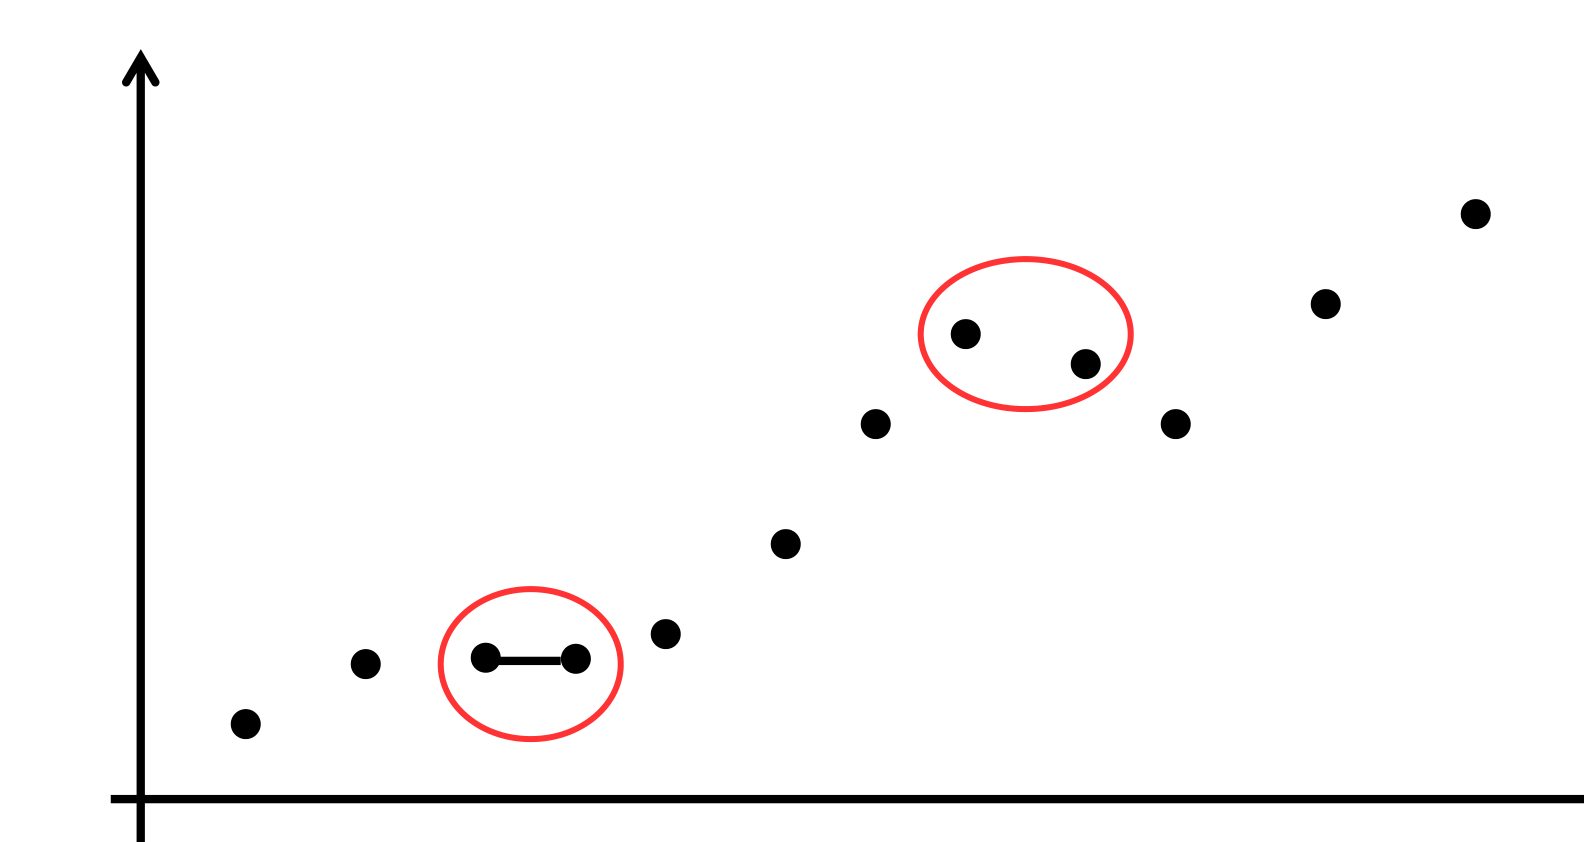
\includegraphics[height=3.8cm,keepaspectratio]{images/slide31_isotonic_step2.png}
  \end{center}
\end{frame}

% Slide 32: PAVA Step 3
\begin{frame}{\rl{الگوریتم تجمیع متجاوزان مجاور: گام ۳}}{\lr{Pool Adjacent Violators: Step 3}}
  \begin{itemize}
    \setlength{\itemsep}{3pt}
    \item ادامه فرآیند تجمیع بلوک‌ها به سمت راست محور متغیر توصیفی.
  \end{itemize}
  \begin{center}
    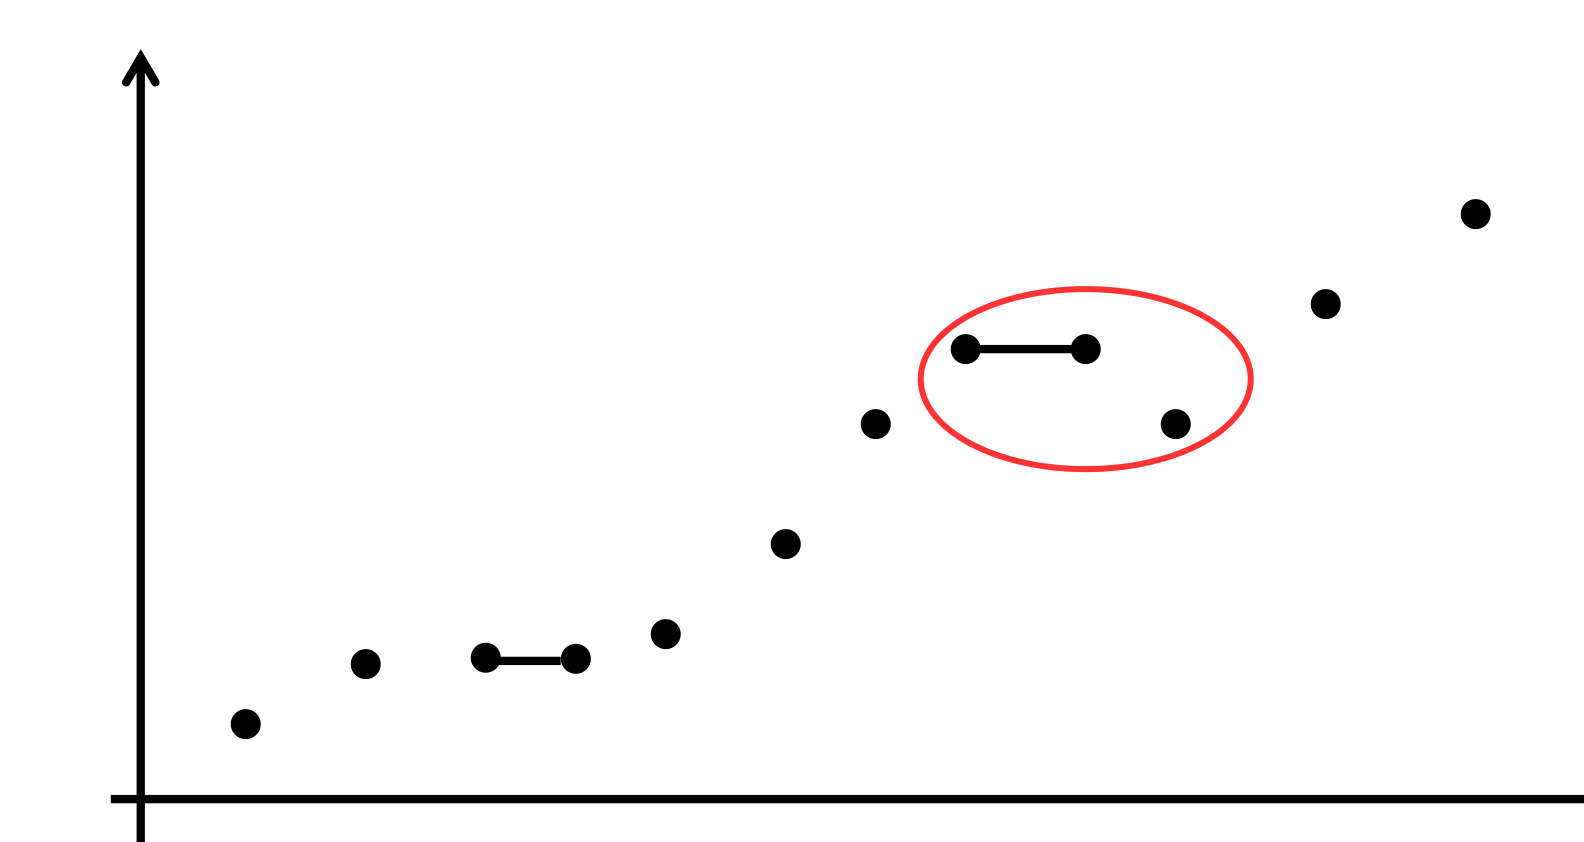
\includegraphics[height=3.8cm,keepaspectratio]{images/slide32_isotonic_step3.png}
  \end{center}
\end{frame}

% Slide 33: PAVA Step 4
\begin{frame}{\rl{الگوریتم تجمیع متجاوزان مجاور: گام ۴}}{\lr{Pool Adjacent Violators: Step 4}}
  \begin{itemize}
    \setlength{\itemsep}{3pt}
    \item آخرین مرحله رفع نقض شرط یکنوایی و برقراری شرط صعودی برای تمام نقاط.
  \end{itemize}
  \begin{center}
    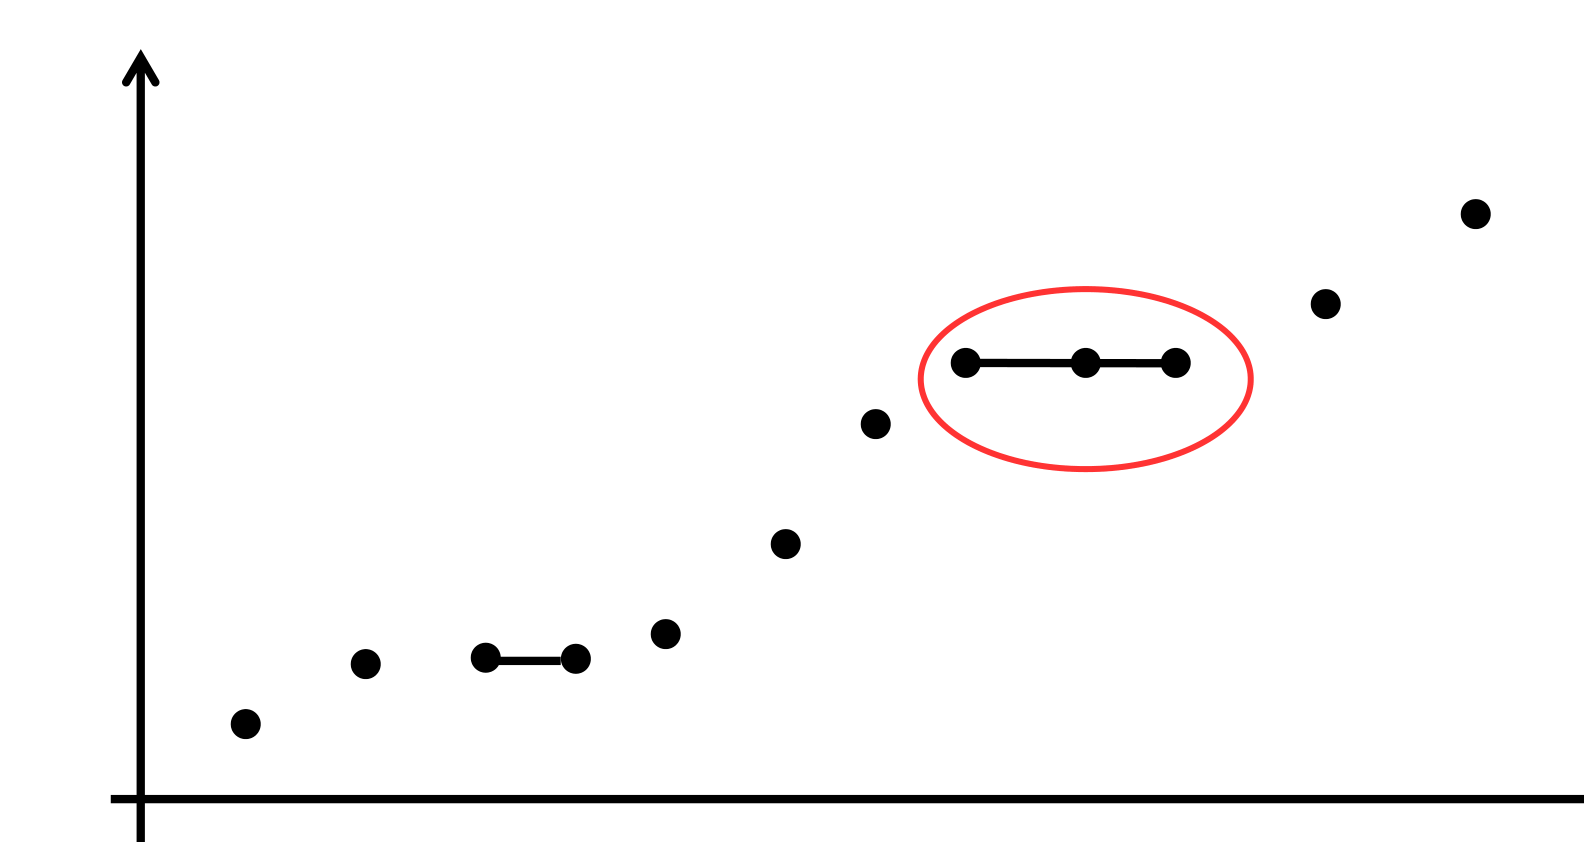
\includegraphics[height=3.8cm,keepaspectratio]{images/slide33_isotonic_step4.png}
  \end{center}
\end{frame}

% Slide 34: PAVA Result Function
\begin{frame}{رگرسیون هم‌نوا: تابع برازش نهایی}{\lr{Piecewise Linear / Step Interpolation}}
  \begin{itemize}
    \setlength{\itemsep}{3pt}
    \item پس از بازآرایی و تجمیع تمامی نقاط به گونه‌ای که شرط یکنوایی برای همه نقاط ارضا شود:
    \item اتصال نقاط حاصل با یک \textbf{تابع تکه‌ای-خطی یا پله‌ای} یکنواخت.
  \end{itemize}
  \begin{center}
    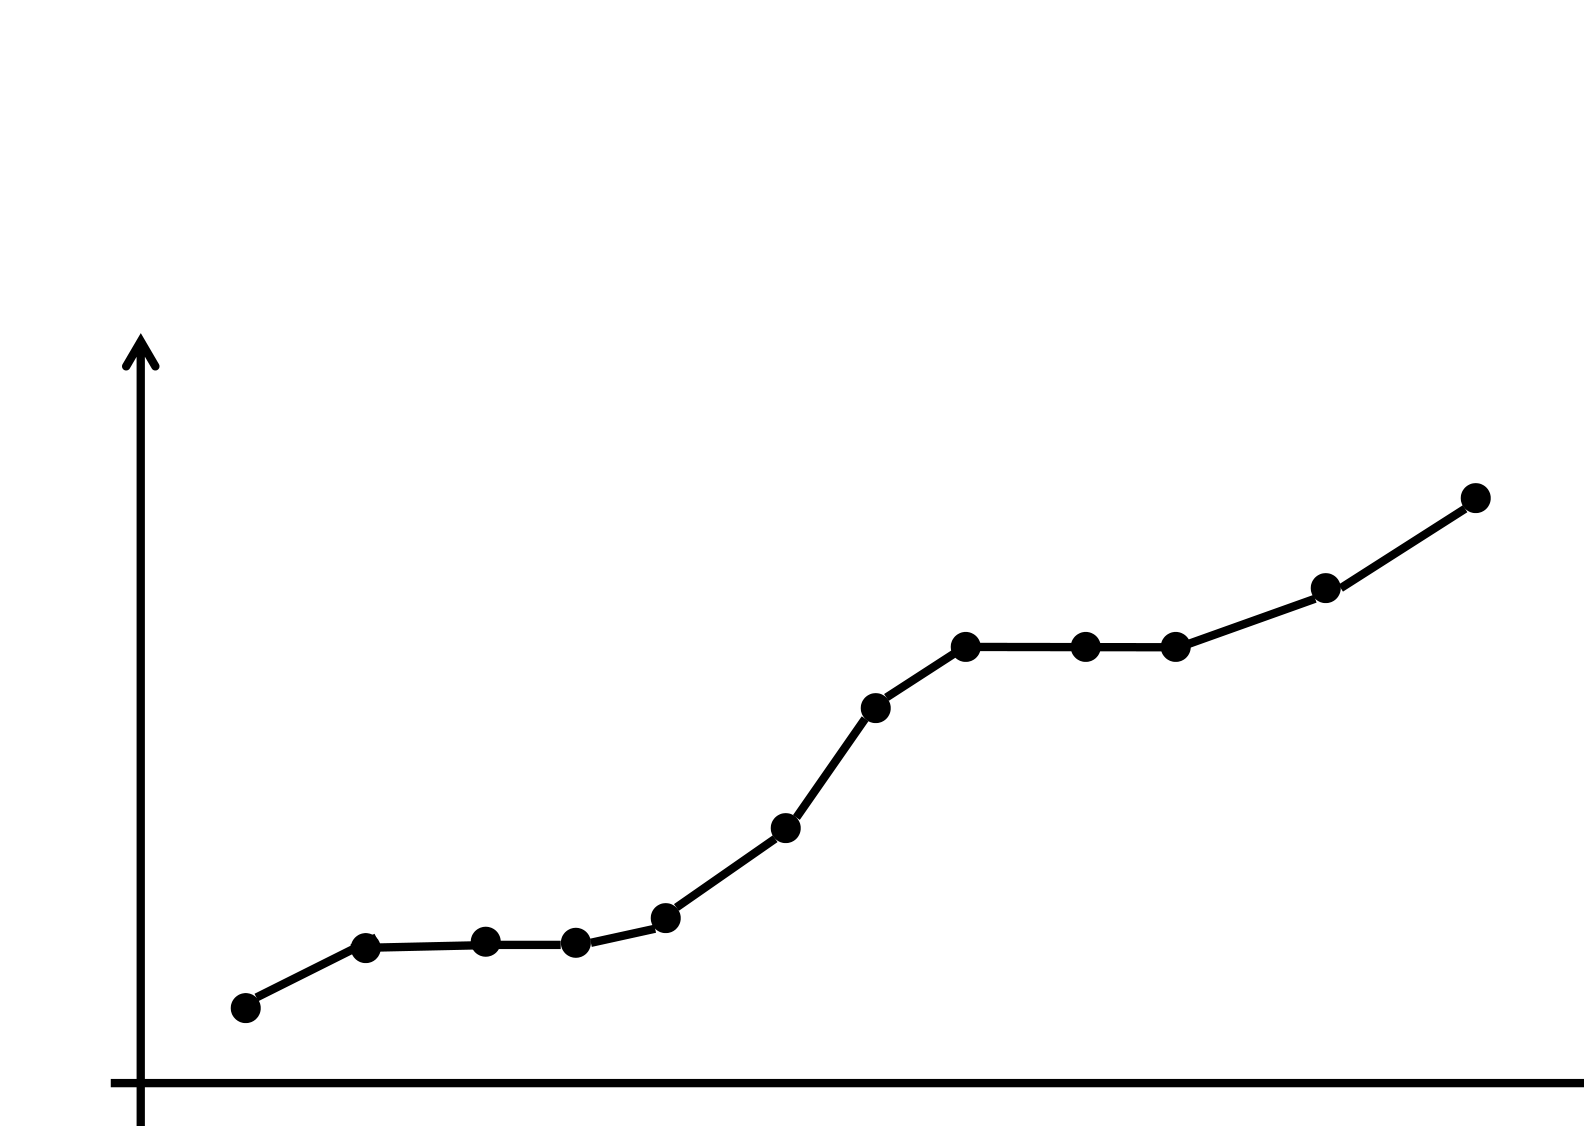
\includegraphics[height=3.6cm,keepaspectratio]{images/slide34_isotonic_step5.png}
  \end{center}
\end{frame}

% Slide 35: PAVA Comparison
\begin{frame}{رگرسیون هم‌نوا: مقایسه با نقاط اصلی}{\lr{Comparison to Original Points}}
  \begin{itemize}
    \setlength{\itemsep}{3pt}
    \item \textbf{تشکیل کفه یا فلات} (\lr{Plateaus})؛ در بخش‌هایی از داده‌ها که اولیه غیریکنواخت بوده‌اند، پله‌های افقی پدید می‌آید.
    \item در عین حال، میانگین مربعات خطا (\lr{MSE}) در کل داده‌ها تحت قید یکنوایی کمینه می‌شود.
  \end{itemize}
  \begin{center}
    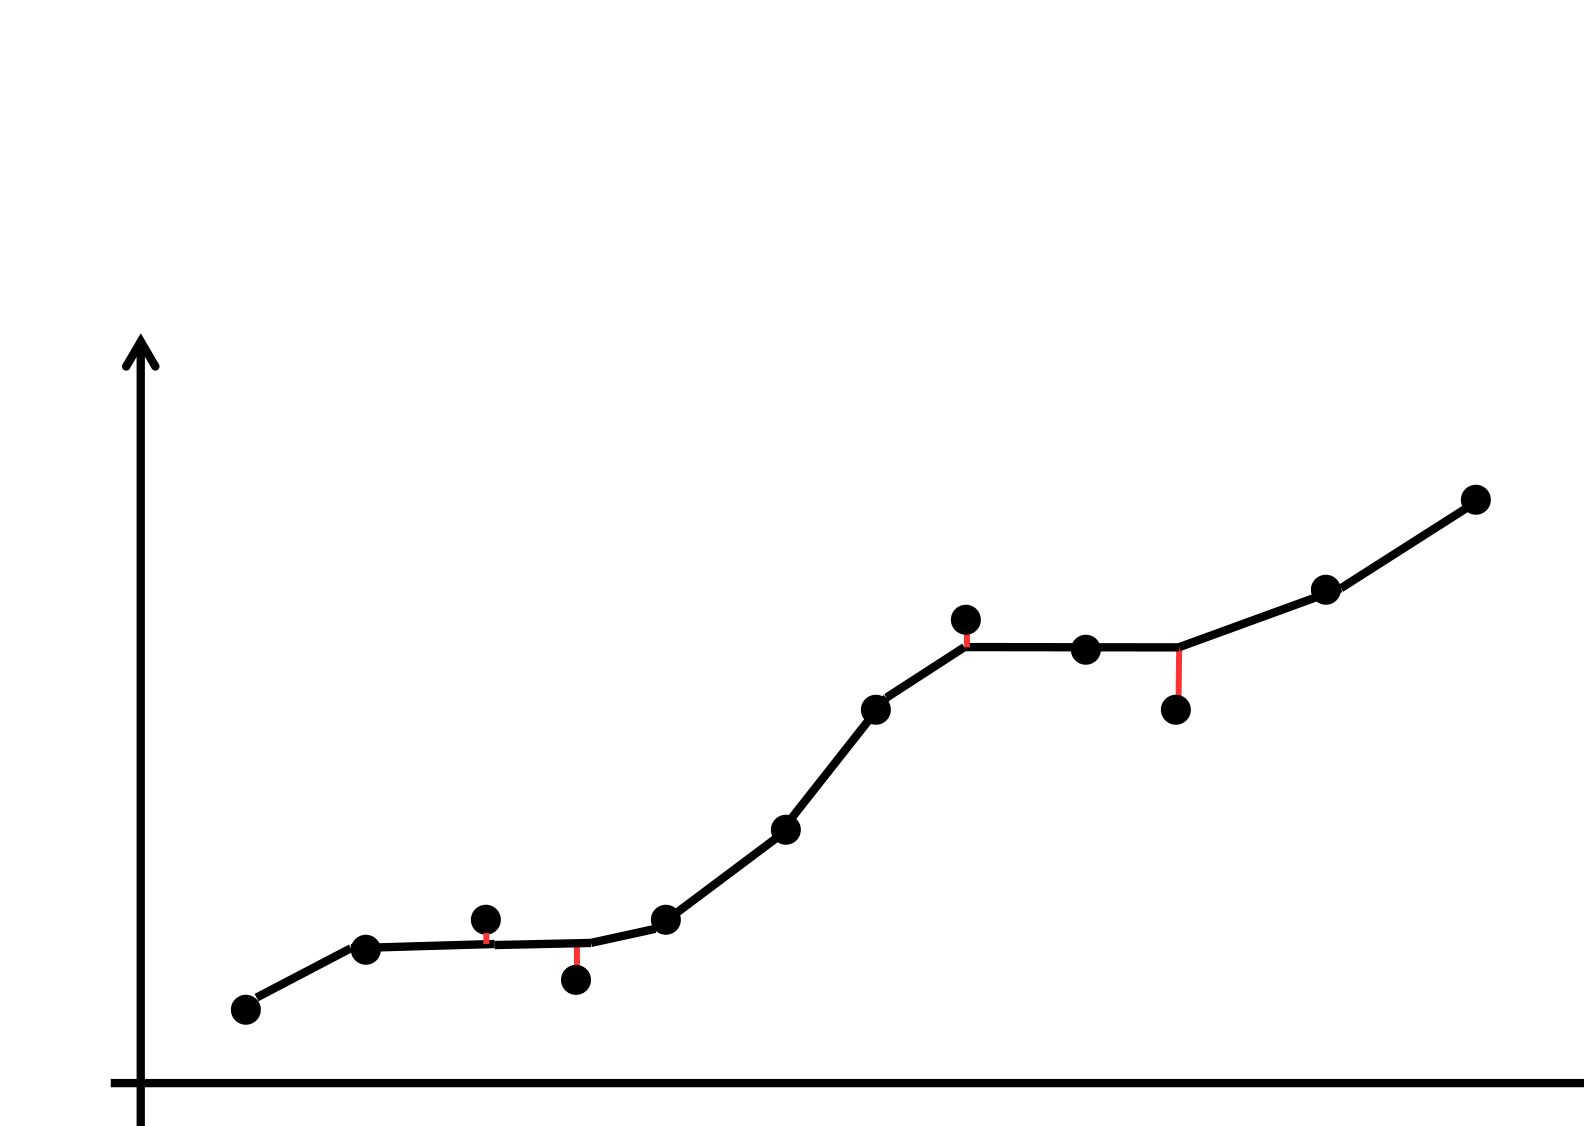
\includegraphics[height=3.6cm,keepaspectratio]{images/slide35_isotonic_step6.png}
  \end{center}
\end{frame}

% Slide 36: Isotonic in Python
\begin{frame}{رگرسیون هم‌نوا در پایتون}{\lr{Isotonic Regression in Scikit-Learn}}
  \begin{itemize}
    \setlength{\itemsep}{4pt}
    \item کتابخانه: \codeinline{from sklearn.isotonic import IsotonicRegression}
    \item \textbf{پارامتر \codeinline{increasing}:}
    \begin{itemize}
      \item \codeinline{True}: قید صعودی یکنواخت | \codeinline{False}: قید نزولی یکنواخت.
      \item \codeinline{'auto'}: تعیین خودکار بهترین جهت بر اساس کمینه‌سازی خطا.
    \end{itemize}
    \item \textbf{پارامتر \codeinline{out\_of\_bounds} (نحوه مدیریت مقادیر نادیده $x$):}
    \begin{itemize}
      \item \codeinline{'clip'}: استفاده از کمترین/بیشترین مقدار $y$ در داده‌های آموزش.
      \item \codeinline{'nan'}: تخصیص مقدار نامعتبر \lr{NaN}.
      \item \codeinline{'raise'}: پرتاب خطا (\lr{Exception}).
    \end{itemize}
  \end{itemize}
\end{frame}

% Slide 37: Non-linear, Non-monotonous
\begin{frame}{مسائل غیرخطی و غیریکنواخت}{\lr{Non-linear, Non-monotonous Problems}}
  \begin{center}
    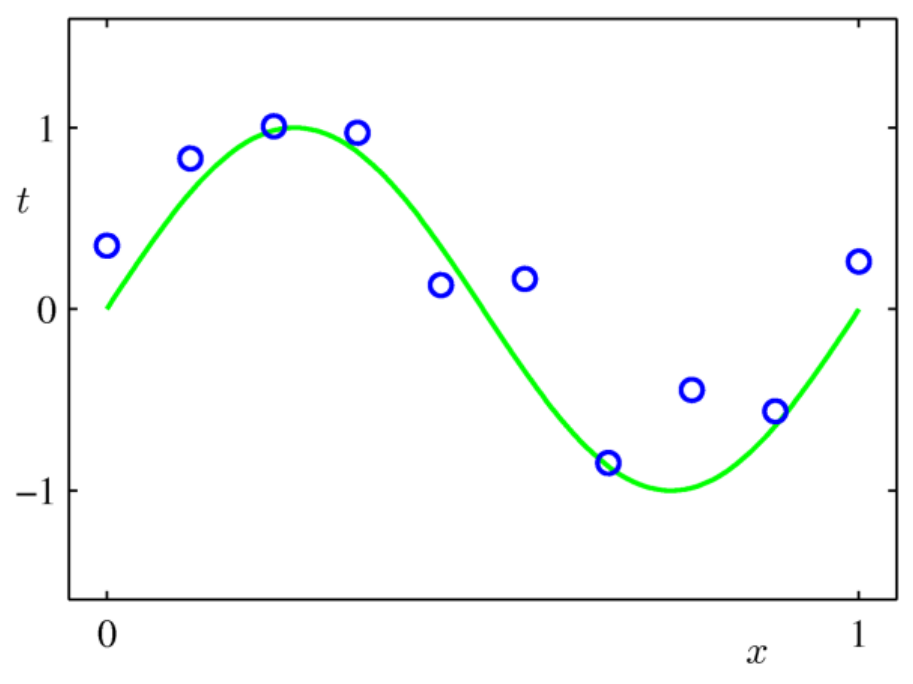
\includegraphics[height=2.7cm,keepaspectratio]{images/slide37_nonmonotone_curve.png}
  \end{center}
  \vspace{-0.2cm}
  \begin{itemize}\setlength{\itemsep}{3pt}
    \item اگر تابع هدف هم غیرخطی و هم غیریکنواخت باشد، چه کنیم؟
    \item \textbf{اعمال تبدیل بر روی متغیرهای توصیفی $X$ به این صورت}:
    \begin{itemize}\setlength{\itemsep}{2pt}\footnotesize
      \item تبدیلات ریاضی مانند $\log(x)$، $\exp(x)$، $\sqrt{x}$، $x^2$ و غیره.
      \item \textbf{تبدیل چندجمله‌ای} (\lr{Polynomial}) به فرم زیر:
      \par\vspace{2pt}\noindent\makebox[\linewidth][c]{$y = w_0 + w_1 x + w_2 x^2 + w_3 x^3$}\par\vspace{2pt}
    \end{itemize}
  \end{itemize}
\end{frame}

% Slide 38: Polynomial Regression
\begin{frame}{رگرسیون چندجمله‌ای}{\lr{Polynomial Regression}}
  \par\vspace{-0.1cm}\noindent\makebox[\linewidth][c]{$\displaystyle \hat{y}(x, \mathbf{w}) = w_0 + w_1 x + w_2 x^2 + \dots + w_d x^d = \sum_{j=0}^d w_j x^j$}\par\vspace{0.2cm}
  \begin{columns}[T]
    \begin{column}{0.58\textwidth}
      \begin{itemize}
        \setlength{\itemsep}{4pt}\small
        \item تعمیم گسترده و پرکاربرد رگرسیون خطی.
        \item برازش همچنان با همان روش کمترین مربعات خطی (\lr{OLS}) صورت می‌گیرد!
        \item \textbf{چالش اصلی:} تمایل شدید به بیش‌برازش در درجات بالای $d$.
        \item \textbf{راهکارها:}
        \begin{itemize}\footnotesize
          \item کاهش درجهٔ $d$
          \item افزایش حجم داده‌های آموزش
        \end{itemize}
      \end{itemize}
    \end{column}
    \begin{column}{0.40\textwidth}
      \begin{center}
        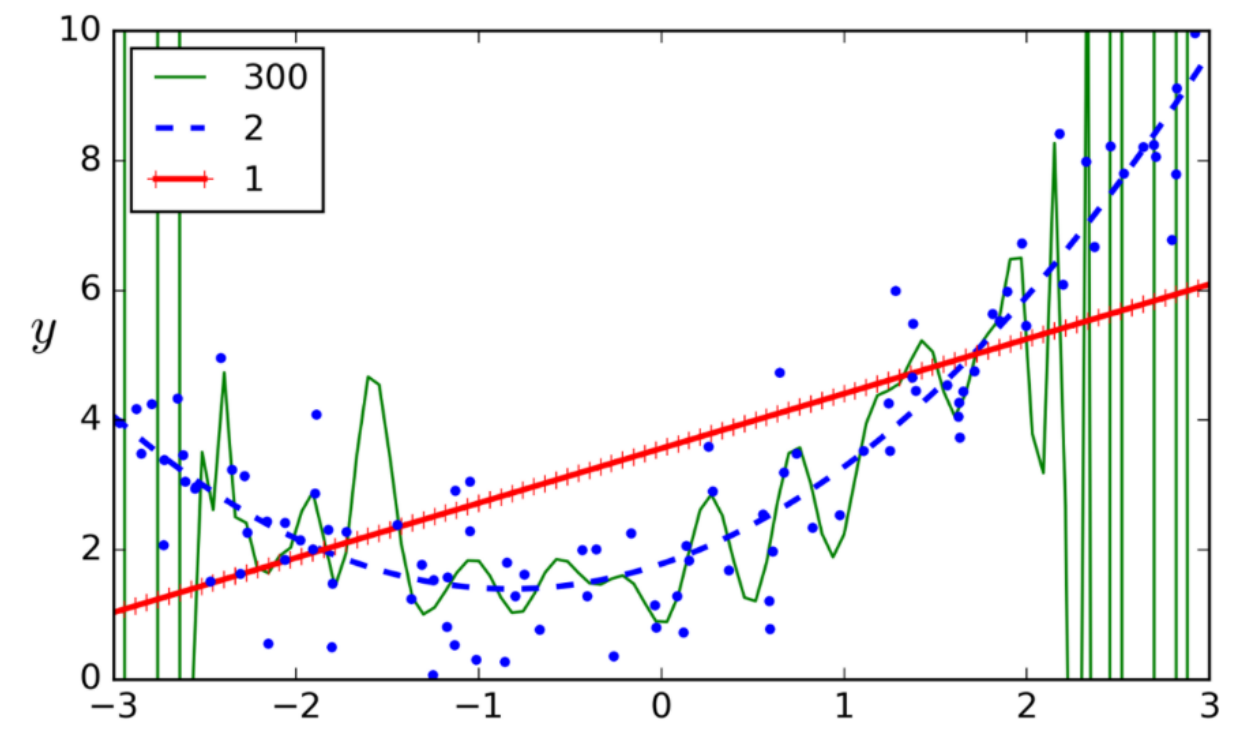
\includegraphics[width=\textwidth,height=3.6cm,keepaspectratio]{images/slide38_polynomial_degrees.png}
      \end{center}
    \end{column}
  \end{columns}
\end{frame}

% Slide 39: Multiple Features Explosion
\begin{frame}{انفجار ابعاد در رگرسیون چندجمله‌ای چندمتغیره}{\lr{Curse of Dimensionality in Polynomial Features}}
  \begin{columns}[T]
    \begin{column}{0.58\textwidth}
      \begin{itemize}
        \setlength{\itemsep}{3pt}
        \item تعداد ویژگی‌های چندجمله‌ای درجهٔ $d$ برای دیتاستی با $f$ ویژگی از مرتبهٔ $\mathcal{O}(f^d)$ رشد می‌کند!
        \item \textbf{مثال با ۳ ویژگی $x, y, z$ و درجهٔ $d=3$}:
        \begin{itemize}
          \setlength{\itemsep}{2pt}
          \item درجهٔ ۲ ($6$ ویژگی): $x^2, y^2, z^2, xy, xz, yz$
          \item درجهٔ ۳ ($10$ ویژگی): $x^3, y^3, z^3, x^2y, \dots$
        \end{itemize}
        \item برای داده‌هایی با ۶۰ ویژگی اولیه، در درجات بالاتر صدها هزار ویژگی جدید پدید می‌آید.
      \end{itemize}
    \end{column}
    \begin{column}{0.40\textwidth}
      \begin{center}
        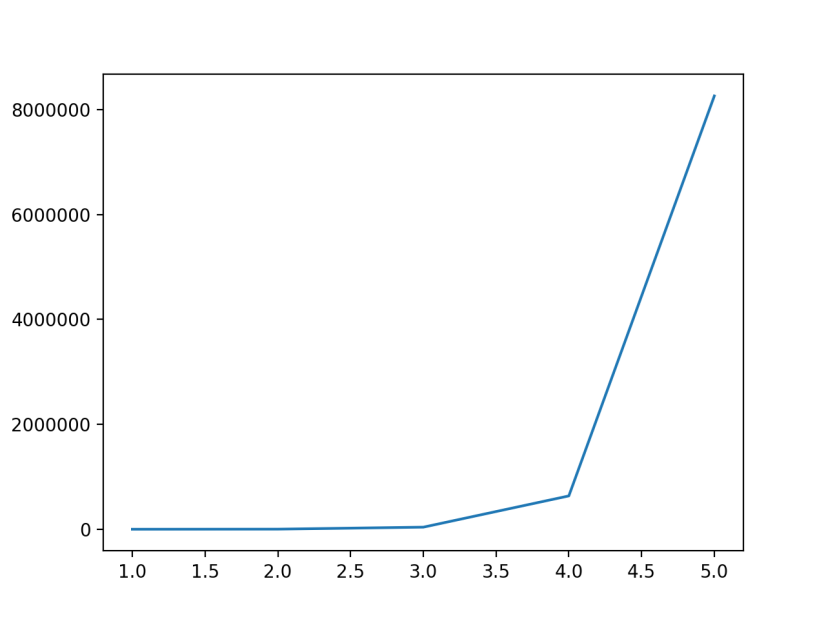
\includegraphics[width=\textwidth,height=4.2cm,keepaspectratio]{images/slide39_feature_explosion.png}
      \end{center}
    \end{column}
  \end{columns}
\end{frame}

% Slide 40: Overfitting in Polynomial
\begin{frame}{رگرسیون چندجمله‌ای و خطر بیش‌برازش}{\lr{Polynomial Regression \& Overfitting}}
  \begin{itemize}
    \setlength{\itemsep}{5pt}
    \item \textbf{چرا مجموعه‌های ویژگی بسیار بزرگ خطرناک هستند؟}
    \item بیش‌برازش را مانند «حفظ کردن» (\lr{Memorization}) داده‌ها در نظر بگیرید.
    \item با ۱۰۰۰ متغیر و ۱۰۰۰ نمونه، مدل می‌تواند هر نمونه را با ترکیب یکتایی از ویژگی‌ها حفظ کند!
    \item اما با ۲ متغیر برای ۱۰۰۰ نمونه، مدل ناچار به «انتزاع» و یادگیری الگوی واقعی می‌شود.
    \item \textbf{قاعده سرانگشتی طلایی:} ابعاد دیتاست هرگز نباید عریض‌تر از طول آن باشد (\lr{Never wider than long})!
  \end{itemize}
  \vspace{0.1cm}
  \begin{center}
    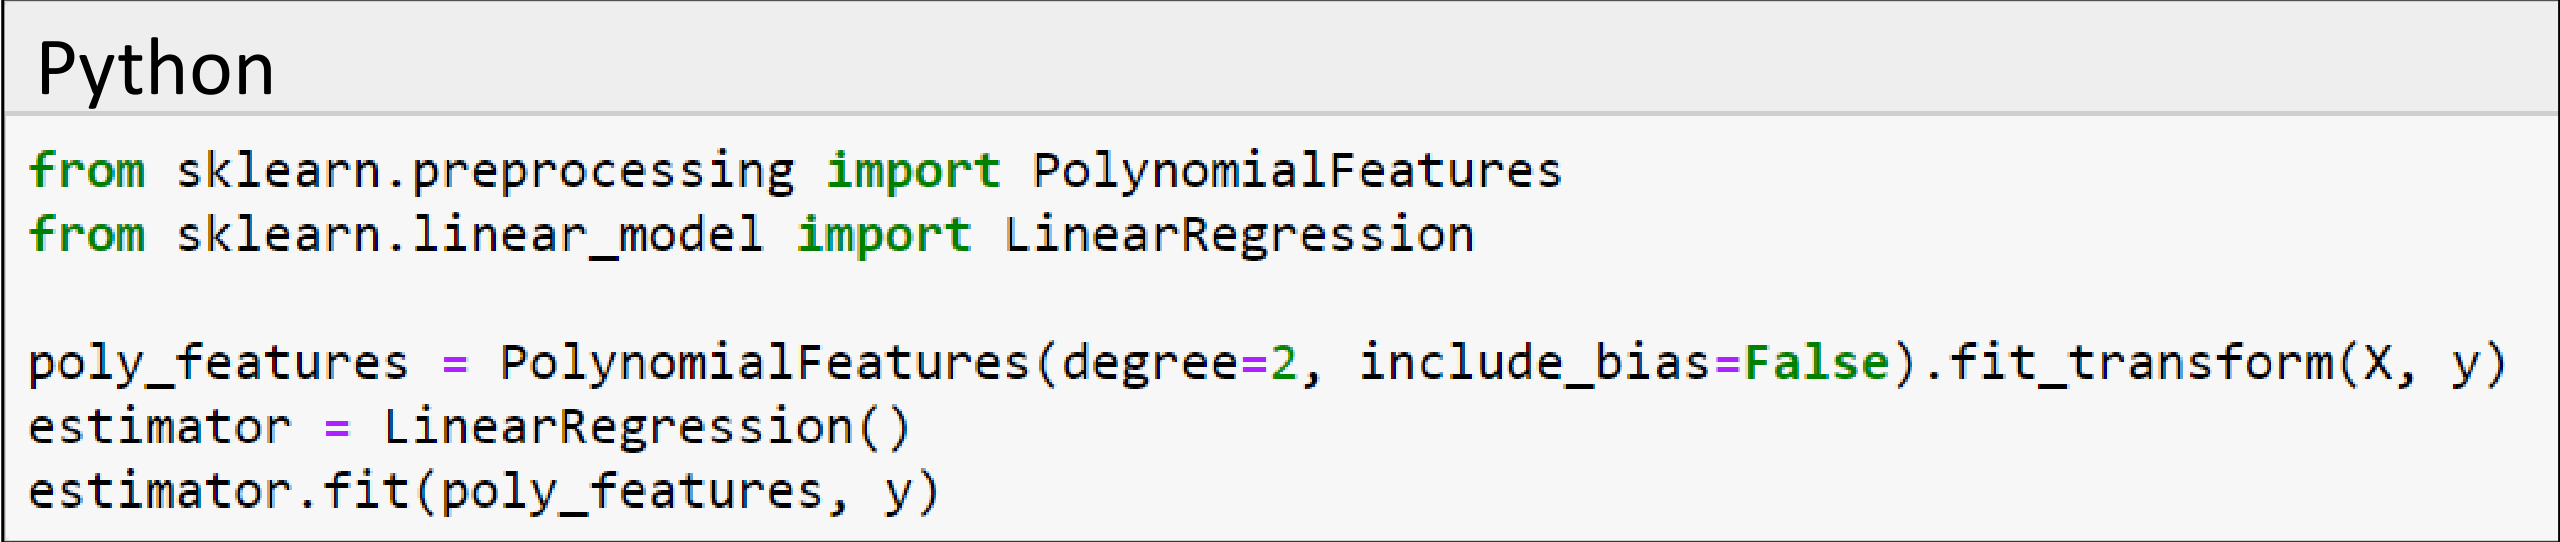
\includegraphics[width=0.85\textwidth,height=2.7cm,keepaspectratio]{images/slide40_polynomial_overfitting.png}
  \end{center}
\end{frame}
